%
% File acl2020.tex
%
%% Based on the style files for ACL 2020, which were
%% Based on the style files for ACL 2018, NAACL 2018/19, which were
%% Based on the style files for ACL-2015, with some improvements
%%  taken from the NAACL-2016 style
%% Based on the style files for ACL-2014, which were, in turn,
%% based on ACL-2013, ACL-2012, ACL-2011, ACL-2010, ACL-IJCNLP-2009,
%% EACL-2009, IJCNLP-2008...
%% Based on the style files for EACL 2006 by 
%%e.agirre@ehu.es or Sergi.Balari@uab.es
%% and that of ACL 08 by Joakim Nivre and Noah Smith

\documentclass[11pt,a4paper]{article}
\usepackage[hyperref]{acl2020}
\usepackage{times}
\usepackage{latexsym}
\renewcommand{\UrlFont}{\ttfamily\small}

\usepackage[utf8]{inputenc}

\usepackage{tabularx}
\usepackage{multirow}
\usepackage{hhline}

\usepackage{xcolor}

\usepackage{cite}
\usepackage[pdftex]{graphicx}
\usepackage{epstopdf}
\usepackage{amsmath}

\usepackage{adjustbox}

 \usepackage{sidecap}
%\usepackage[innercaption]{sidecap}
\sidecaptionvpos{figure}{c}

\newcommand{\argmax}[1]{\underset{#1}{\operatorname{arg}\,\operatorname{max}}\;}
\newcommand{\argmin}[1]{\underset{#1}{\operatorname{arg}\,\operatorname{min}}\;}
\usepackage{bbm}
\usepackage{amsfonts}
\newcommand{\indicator}{\ensuremath{\mathbbm{1}}}

% This is not strictly necessary, and may be commented out,
% but it will improve the layout of the manuscript,
% and will typically save some space.
\usepackage{microtype}



%\aclfinalcopy % Uncomment this line for the final submission
%\def\aclpaperid{***} %  Enter the acl Paper ID here

%\setlength\titlebox{5cm}
% You can expand the titlebox if you need extra space
% to show all the authors. Please do not make the titlebox
% smaller than 5cm (the original size); we will check this
% in the camera-ready version and ask you to change it back.

\newcommand\BibTeX{B\textsc{ib}\TeX}

\title{Bidirectional imparting of word embeddings for interpretability enhancement and gender debiasing}

\author{Lütfi~Kerem~Şenel$^1$ \And Furkan~Şahinuç$^2,3$ \And Veysel~Yücesoy$^2$ \And Hinrich~Schütze$^1$ \And Tolga~Çukur$^3$ \And Aykut~Koç$^3$\\
  $^1$Center for Information and Language Processing, LMU Munich, Germany \\
  $^2$ASELSAN Research Center, Ankara, Turkey \\
  $^3$Electrical and Electronics Engineering Department, Bilkent University, Ankara, Turkey
  \texttt{\{lksenel,furkansahinuc19,veyselyucesoy\}@gmail.com}\\
  \texttt{inquiries@cislmu.org, aykut.koc@bilkent.edu.tr, cukur@ee.bilkent.edu.tr } \\}

\date{}

\begin{document}
\maketitle
\begin{abstract}
Word embeddings, which enable mapping of semantic properties of words into a dense vector space, typically suffer from poor interpretability - a general deficiency in many neural learning models. 
Here, we propose a generalized method for aligning embedding dimensions with concepts during the learning phase to impart interpretability while preserving the inherent semantic structure. 
The proposed method separately utilizes both directions of each vector space dimension to increase the number of imparted concepts.
Experiments are performed on the scalable \textit{word2vec} algorithm.
% while concepts are extracted from two different lexical resources, Roget's Thesaurus and \textit{WordNet}, to demonstrate generalizability. 
Comprehensive demonstrations clearly indicate that bidirectional imparting allows for higher interpretability without sacrificing performance evaluated on intrinsic tests as well as several downstream classification tasks.
Moreover, we adopt the imparting method for reducing gender bias in word embedding models. Specifically, we show that efficacy of current debiasing methods can be enhanced by encoding gender opposite concepts (e.g., male-female) in a single embedding dimension as evaluated using intrinsic bias evaluations as well as fairness measurements for high level classification tasks.
%Finally, we introduce a hybrid gender- and interpretability-imparted model that simultaneously achieves gender debiasing and interpretability without compromising task performance.
\end{abstract}

\section{Introduction}\label{sec:intro}

Continuous dense vector representations of words, i.e., \emph{word embeddings} \citep{mikolov13word2vec_a,mikolov13word2vec_b,pennington14glove,bojanowski2017enriching}, are useful tools to capture semantic and syntactic features of language. 
%Word embeddings offer performance benefits in a variety of natural language processing (NLP) tasks including named entity recognition \citep{habibi2017deep,sienvcnik15NER} sentiment analysis \citep{tang2014learning,yu17sentiment}, semantic text similarity \citep{kenter15textSimilarity}. Moreover, e
Embeddings have demonstrated use in a broad domain of applications that involve lexical semantics. In the neuroscience domain, they can be employed to map semantic representations across cortex \citep{ruan16brainActivity,huth16semanticMaps}, to develop a decoder that extracts linguistic meaning from measured brain activity \citep{pereira18universalDecoder}, or to detect incoherent speech for diagnosing schizophrenia \citep{iter2018automatic}. In the social domain, word and sentence embeddings can be used to analyze public polarization in social media \citep{demszky19analyzing}. In evolutionary linguistics, word embeddings enable tracking the history of changes in word meaning over the course of years \citep{hamilton16diachronic}. Recent studies suggest that embeddings also enable efficient capture and quantification of gender and ethnic stereotypes and biases in language \citep{bolukbasi16debiasing,garg18gender100years,caliskan17humanLikeBiases} and their evolution across time \citep{agarwal2019word}. Embeddings can also be used to quantify the semantic similarity between different languages \citep{senel17crossLingual,senel18atlas}.

%Significant performance improvements in common NLP tasks along with utility in related domains led to growing popularity for word embedding models. 
Despite extensive efforts in developing improved models \citep{yu2017refining, celikyilmaz15enriching, yu14improving, liu15learning, mrksic16counterFitting, bollegala16joint, yang16fineTuning}, a central limitation is the lack of interpretability for semantic concepts represented by individual dimensions of the dense vector spaces \citep{chen16InfoGAN,levy14dependency}. Generally, the learned embeddings make sense only in relation to each other and their specific dimensions cannot be interpreted explicitly. Interpretability is a highly desired trait for word embeddings for several reasons. Word embeddings serve as an initial stage in many deep learning models for NLP tasks, so their interpretability can be key to attaining interpretable deep learning models. The ability to interpret an embedding model would unravel the semantic concepts represented along the vector space dimensions. In turn, this information can be leveraged to remove redundant or irrelevant dimensions from the embedding model to optimize performance in a given task, reducing computation and memory requirements. This can also facilitate removal of unwanted biases from the embedding such as gender information \citep{dufter19ultraDense}. 

% Previous studies have put forth several important approaches to address limitations on interpretability of word embeddings. A group of studies proposed to use sparsity constraints such as non-negative matrix factorization \citep{murphy12nnse,luo15online,fyshe14interpretable}, sparse coding \citep{arora18linalg,faruqui15sparse} and sparse auto-encoders \citep{subramanian18spine} that yield sparse word representations. Since each word is represented by only a few dimensions, it is easier to understand what semantic features the dimensions capture.
% However, larger vocabulary requires higher dimensionality to achieve a desired sparsity level which increases memory and computation requirements. Another group of studies proposed to instead use orthogonal transformations over the high performing dense embeddings \citep{zobnin17rotations,park17rotated,dufter19ultraDense} in order to preserve task performance. Yet, the level of improvement in interpretability that orthogonal transformations can achieve is relatively limited. 
In a recent study, imparting approach was proposed to obtain interpretable word embeddings while still preserving internal semantic structure \citep{senel20impart}. The objective function of GloVe embedding algorithm \citep{pennington14glove} was modified to align each individual dimension of the vector space with a single pre-defined concept. However, this unidirectional imparting of embedding dimensions does not utilize the full capacity of the embedding space since negative directions are ignored. Moreover, generalizability of the imparting method beyond GloVe algorithm was not investigated.

In this study, we introduce a generalized imparting approach that is capable of online learning and bidirectional imparting. The proposed method utilizes both directions along each dimension of the vector space separately to encode two different concepts, which can be chosen arbitrarily or chosen as opposites (e.g., \textit{good} - \textit{bad}, \textit{male} - \textit{female}) as a special case. Since our imparting method can encode any concept to any direction of any embedding dimension, it provides more efficient use of the embedding space while increasing encoding flexibility. The proposed method is demonstrated on the skip-gram model of the word2vec method \citep{mikolov13word2vec_a,mikolov13word2vec_b}, where several lexical resources are leveraged to select concepts. Specifically, Roget's Thesaurus and a more contemporary lexical database \textit{WordNet} are examined. The relative weighting of interpretability versus semantic structure is controlled by a parameter that is selected to optimize the trade-off between interpretability and task performance. Comprehensive experiments are performed to demonstrate improved interpretability for word embeddings, without significant performance loss. Performance is evaluated using intrinsic tests (i.e., word similarity and word analogy) as well as several downstream classification tasks. Inspired by the results in \citep{bolukbasi16debiasing}, we also demonstrate that bidirectional imparting can concentrate gender information in a single embedding dimension as a continuum. As a result, it enables efficient capture of gender bias and debiasing through removal of the relevant embedding dimension. 
% \textcolor{black}{The main contributions of the current study are summarized below:}

% \begin{itemize}
%     \item \textcolor{black}{We provide the first demonstration of imparting to the word2vec model to achieve interpretable embedding models in an online algorithm without sacrificing task performance.}

%     \item \textcolor{black}{We introduce for the first time a bidirectional imparting method that can encode arbitrary concepts to positive and negative directions of embedding dimensions.}

%     \item \textcolor{black}{We demonstrate that the bidirectional imparting of arbitrary concepts offers superior performance compared to encoding of polar opposites to each embedding dimension, in terms of interpretability, intrinsic and downstream evaluation tasks.}

%     \item \textcolor{black}{We propose for the first time an imparting method to concentrate gender information to a designated embedding dimension, along with a hybrid method that achieves concurrent gender and interpretability imparting.}

%     \item \textcolor{black}{We demonstrate that gender-imparted embedding models improve performance of gender debiasing methods, in terms of gender bias metrics  and high-level evaluation tasks.}
% \end{itemize}

% The organization of the paper is as follows: In Section \ref{sec:related},  we discuss previous studies focusing on interpretability of word embeddings. In Section \ref{sec:methods}, introduce the proposed generalized imparting method and a new interpretability metric. We also describe the application of imparting for gender debiasing in the same section. We present our results in Section \ref{sec:results} and finally, we conclude the paper in Section \ref{sec:concl}.

\section{Related Work} \label{sec:related}

Benefits of interpretable word embeddings have motivated several previous efforts on developing methods to improve interpretability. Majority of these studies introduce a sparsity constraint in order to learn sparse representations where each word is represented by only a few non-zero dimensions. 
%The motivation behind sparsity is that by investigating the words that correspond to non-zero values in a dimension, one might infer which semantic features are encoded in that dimension. 
Based on this idea, a method called non-negative sparse embeddings (NNSE) was proposed to perform non-negative matrix factorization (NMF) on word co-occurrence variant matrices \citep{murphy12nnse}. As an extension to NNSE, \citet{fyshe14interpretable} proposed joint non-negative sparse embedding (JNNSE) to incorporate additional knowledge on word similarity as measured by the similarity of cortical activity patterns they evoked. To address the memory and scale issues of the NNSE based methods, \citet{luo15online} proposed an online learning method, where sparse embeddings were obtained using a modified skip-gram model \citep{mikolov13word2vec_a}. Several other studies proposed to learn sparse transformations that map pre-trained state-of-the-art embeddings to sparse, more interpretable vector spaces instead of learning them from corpora (or co-occurrence matrices) directly. \citet{arora18linalg} and \citet{faruqui15sparse} used sparse coding methods and \citep{subramanian18spine} proposed to train a sparse auto-encoder.

% While the above-mentioned approaches can increase interpretability to a certain degree, they do not exercise control over the specific concepts or word senses that are captured in the embedding dimensions.  
% Inspired by research in topic modelling, \citep{panigrahi19word2sense} proposed a method based on Latent Dirichlet Allocation (LDA) to extract the distributions of difference word senses from a corpus, which are then used to learn sparse interpretable word embeddings in a method named Word2Sense. 
% Note that most previous studies on incorporation of topic modeling to word embedding primarily prioritize the coherence of learned topics as opposed to interpretability of individual embedding dimensions \citep{blei03LDA,liu15topical,moody16mixing,das15gaussian,shi17jointly}.
% Therefore, these methods are not considered further in this study.

Sparse representations typically have higher dimensionality than dense embeddings since only few words are encoded in each dimension. Thus, they can suffer from memory and scale issues especially for tasks that require a broad vocabulary. 
% Moreover, the increased dimensionality can also yield suboptimal performance in NLP tasks such as word analogy \citep{senel20impart}. 
To strictly preserve the dimensionality and semantic structure of word embeddings, several researchers proposed orthogonal instead of sparse transformations. In \citet{park17rotated}, rotation algorithms based on exploratory factor analysis (EFA) with orthogonality constraints were experimented. In \citet{zobnin17rotations}, orthogonal transformations were used to improve clustering of words along individual embedding dimensions. However, increases in clustering along a subset of embedding dimensions come at the expense of reduced clustering (i.e., interpretability) along remaining dimensions \citep{zobnin17rotations}. In \citet{dufter19ultraDense}, orthogonal transformations were used to align a given linguistic signal (i.e., collection of words) to an embedding dimension in order to obtain an interpretable subspace. However, this method has only been demonstrated in a unidimensional subspace to date, so its performance in higher dimensional subspaces remains unclear. In a concurrent, independent study \citep{mathew20polar}, a transformation method, \textit{POLAR}, was proposed to map an existing embedding space to a polar space where each embedding dimension corresponds to a pair of antonyms (i.e. polar opposites).
% With the exception of \citep{fyshe14interpretable}, \citep{dufter19ultraDense} and \citep{mathew20polar}, the prior art discussed in this section does not incorporate or else leverage lexical information from external resources. In two recent studies, we have leveraged external lexical resources to propose a quantitative metric of interpretability for embedding models \citep{senel18semanticStructure}, and then to impart interpretability during the learning phase to maintain model performance \citep{senel20impart}. 
In a recent study \citep{senel20impart}, imparting method was proposed in which individual dimensions of the model were aligned with concepts defined a priori based on the external resource. Despite its success, the previous imparting method was demonstrated only for the off-line GloVe method, and only the positive direction of each dimension was matched up with a concept. 
%This unidirectional imparting limits the representational capacity of the resulting embedding for semantic concepts, and does not allow for continuous encoding of opposing concepts. 

\section{Methods} \label{sec:methods}

%In this section, we introduce the generalized bidirectional imparting method and an interpretability evaluation method for bidirectional embeddings. We also discuss the application of bidirectional imparting on gender bias.

\subsection{Generalized Bidirectional Imparting }
\label{sec:gen_imparting}

A unidirectional method was introduced in \citep{senel20impart} by modifying the cost function of the GloVe algorithm to align predefined concepts (i.e., word-groups) with individual embedding dimensions. This modified cost is given as:
\begin{align}
\begin{split}
	 &\sum_{i,j=1}^{V} f(X_{ij}) \Bigg[ \left(\vec{w}_i^T\vec{\tilde{w}}_j + b_i + \tilde{b}_j -\log{}X_{ij}\right)^2 \\
	      & +\: k^g\left(\sum_{c=1}^{C} \indicator_{i\in{}F_c} \: g(w_{i,c}) + \sum_{c=1}^{C} \indicator_{j \in F_c} \: g(\tilde{w}_{j,c})  \right) \Bigg] 
\end{split}
\label{eq:glove_uni}
\end{align}
where $\vec{w}_i$ and $\vec{\tilde{w}_j}$ denote word and context vectors, $w_{i,c}$ and $\tilde{w}_{j,c}$ denote $c^{th}$ components of word and context vectors, $b_i$ and $\tilde{b}_j$, denote word and context biases, $X_{ij}$ denotes co-occurrence for $i^{th}$ and $j^{th}$ words in vocabulary, $V$ denotes vocabulary size, and $f(\cdot)$ is a weighting function to prevent bias from rare words. The first term in the cost aims to encapture semantic structure in the embedding model based on word co-occurences. Meanwhile, the second term aims to align embedding dimensions with word-groups. In this latter term, $C$ denotes the number of word-groups (where $C\leq dim(\vec{w})$), $\indicator_{x \in S}$ is the indicator variable for the inclusion ${x \in S}$, $F_l$ denotes the indices of words that belong to the $l^{th}$ group, $k_g$ controls the relative weighting of the second term, and the function $g(\cdot)$, adjusts the size of the updates during training. 
% $g(\cdot)$ is defined as:
% \begin{equation*}
%     g(x) = 
%     \begin{cases} 
%     1/2\cdot exp(-2x), & \text{if}~x<0.5 \\
%     ~1/(4ex), & \text{otherwise}
%     \end{cases}
% \end{equation*}

In this study, we propose a generalized imparting framework that is capable of online learning and bidirectional imparting. To alleviate computation and memory limitations, we focus on the skip-gram model of word2vec with negative sampling.
% The objective that the skip-gram model aims to maximize for a word pair $(i, j)$ is given as:
% \begin{equation}
%     \log ~ \sigma ({\vec{\tilde{w}}_{j}}^T \vec{w}_{i}) + \sum_{t = 1}^{m} {\mathbb{E}}_{z_t \sim P_n(w)} \bigg[ log ~ \sigma({\vec{-\tilde{w}}_{z_t}}^T \vec{w}_{i}) \bigg]   
%     \label{eq:word2vec}
% \end{equation}
% where $\sigma$ is the sigmoid function, $m$ is number of negative samples and $P_n(w)$ is the unigram distribution ($U(w)$) raised to the power 3/4, $E[\cdot]$ is the expectation operation and $z_t$ is the index of the word from the $t^{th}$ draw from the unigram word distribution. 
% A significant difference between word2vec and GloVe algorithms is that word2vec does not require a global co-occurrence matrix. Rather, it updates word vectors in an online manner by sliding a window through the corpus. In the word2vec algorithm, word vectors $\vec{w}_{i}$ and $\vec{w}_{j}$ are updated whenever $j^{th}$ word occurs in $i^{th}$ word's context as the algorithm iterates over the corpus. Therefore, the training process of the word2vec algorithm consists of many small and noisy updates. On the other hand, in the GloVe algorithm, iterations are performed over the weighted global cooccurrence matrix and word vectors $\vec{w}_{i}$ and $\vec{w}_{j}$ are updated only once in an epoch based on their cooccurrence, but the magnitude of the update depends on their overall cooccurrence count. Therefore, GloVe consists of fewer, but less noisy updates compared to word2vec.
Although the learning mechanisms of GloVe and word2vec are different, unidirectional imparting can still be implemented by the following modified objective:
\begin{align}
\begin{split}
log ~ & \sigma ({\vec{\tilde{w}}_{j}}^T \vec{w}_{i}) + \sum_{t = 1}^{m} {\mathbb{E}}_{z_t \sim P_n(w)} \bigg[ log ~ \sigma({\vec{-\tilde{w}}_{z_t}}^T \vec{w}_{i}) \bigg] \\ 
& -k^w \Bigl(  \sum_{c=1}^{C} \indicator_{i\in{}F_c} \: g(w_{i,c}) + \sum_{c=1}^{C} \indicator_{j \in F_c} \: g(\tilde{w}_{j,c}) \Bigr)
\end{split}
\label{eq:word2vec_uni}
\end{align}
where $\sigma$ is the sigmoid function, $m$ is number of negative samples and $P_n(w)$ is the unigram distribution ($U(w)$) raised to the power 3/4, $E[\cdot]$ is the expectation operation and $z_t$ is the index of the word from the $t^{th}$ draw from the unigram word distribution.
%In the additional term in \eqref{eq:word2vec_uni}, $C$ denotes the number of word-groups ($C\leq dim(\vec{w})$), $F_c$ denotes the indices of words that belong to the $c^{th}$ group, $k_w$ controls the relative weighting of the second term, and function $g(\cdot)$, adjusts the size of the updates during training. 
Although the additional terms in \eqref{eq:glove_uni} and \eqref{eq:word2vec_uni} look identical, throughout the training process, their relative influence over the original embedding loss can be significantly different. To account for these differences, different weighting factors $k^g$ and $k^w$ are defined.  

Imparting achieves enhanced interpretability in word embeddings by enforcing words related to predefined concepts to project more strongly onto individual embedding dimensions. However, imparting was previously only performed for the positive direction of embedding dimensions. As discussed in \citep{senel18semanticStructure}, negative directions are equally suitable to encode semantic, interpretable concepts. Based on this argument, in this study, we extend the imparting method to both directions of the embedding dimensions. 
%\textit{Bidirectional imparting} allows us to double the number of concepts that can be encoded. 
%Although one can double the embedding dimension for the unidirectional case to cover same number of concepts, this will increase model complexity and unnecessarily cause additional computational costs. 
Given a fixed number for embedding dimension, \textit{bidirectional imparting} doubles the concept capacity with respect to the unidirectional case. Moreover, by encoding opposite concepts such as \textit{good} and \textit{bad} or \textit{male} and \textit{female} to opposing directions of the same dimension, these concepts can be represented in a continuum.

The proposed objective for the bidirectionally imparted word2vec model is as follows:
\begin{align}
\begin{split}
& log ~ \sigma ({\vec{\tilde{w}}_{j}}^T \vec{w}_{i}) + \sum_{t = 1}^{m} {\mathbb{E}}_{z_t \sim P_n(w)} \bigg[ log ~ \sigma({\vec{-\tilde{w}}_{z_t}}^T \vec{w}_{i}) \bigg] \\ 
& -k^w \Bigl(  \sum_{c=1}^{C^+} \indicator_{i\in{}F^+_c} \: g(w_{i,c}) + \sum_{c=1}^{C^+} \indicator_{j \in F^+_c} \: g(\tilde{w}_{j,c}) \\
& ~~~~~ - \sum_{c=1}^{C^-} \indicator_{i\in{}F^-_c} \: g(w_{i,c}) - \sum_{c=1}^{C^-} \indicator_{j \in F^-_c} \: g(\tilde{w}_{j,c}) \Bigr)
\end{split}
\label{eq:word2vec_bi}
\end{align}
where $C^+$ and $C^-$ are the number of word-groups associated with positive and negative directions respectively ($C^+ \leq dim(\vec{w})$, $C^- \leq dim(\vec{w})$). $F^+_c$ and $F^-_c$ denote the indices of words that belong to the $c^{th}$ group in the positive and negative directions, respectively. 

Here word-groups encoded in opposing directions of a given dimension are referred to as word-group pairs. Ideally, the word-group pairs should not contain overlapping words  ($F^+_c \cap F^-_c = \emptyset ~~\forall c$) to prevent weak word representations. In practice, this problem can be alleviated by rearrangement of word-group pairs. In this study, we applied a simple rearrangement procedure to prevent overlap. For a given embedding dimension, we first selected two random word-groups. When overlap was present between the two word-groups, the second word-group was reselected from the set of remaining unpaired groups. This procedure was iterated until all word-groups were paired\footnote{For cases when word-groups have a substantial proportion of overlapping words, more sophisticated matching algorithms might be necessary. However, here, we were able to find a non-overlapping pairing after few trials (less than 5)}.

\subsection{Interpretability Evaluation}
\label{sec:interp_eval}

% Interpretability of word embeddings is traditionally evaluated using the \textit{word intrusion} test \citep{chang09wordintrusion}. In this test, for a given embedding dimension, human evaluators are asked to distinguish an intruder word that is randomly selected from the lower half of the dimension (and is also among the top 10\% in another dimension) from the top 5 words in that dimension. In practice, the word intrusion test suffers from heavy experimental burden and limited reproducibility, especially for embedding models with hundreds of dimensions. Therefore, an alternative automated method was used in \citep{senel20impart} to measure interpretability based on a pre-defined collection of word categories, SEMCAT \citep{senel18semanticStructure}, that has been shown to correlate well with evaluations based on word intrusion \citep{senel20impart}. This method is extended to consider subcategories in \citep{senel18trInterpret}.

Interpretability of word embeddings is traditionally evaluated using the \textit{word intrusion} test \citep{chang09wordintrusion}.
Due to its advantages over word intrusion test in terms of scalability and reproducibility, here we adapt the interpretability evaluation based on SEMCAT categories \citep{senel18semanticStructure}. However, the interpretability metric that is introduced in \citet{senel18semanticStructure} and later improved in \citet{senel18trInterpret}, cannot capture the difference between interpretability changes in the positive and negative directions of an embedding dimension, because it performs maximum pooling over the opposite directions of each dimension. To enable sensitive capture of this information, here we proposed a new directional interpretability metric:
\begin{equation} \label{eq:interpretability_new}
\begin{split}
&IS^+_{l,k} = \max_{n_{min} \leq n \leq n_c } \frac{|S_c \cap V^+_l(\lambda \times n)|}{n} \times 100  \\
&IS^-_{l,k} = \max_{n_{min} \leq n \leq n_c } \frac{|S_c \cap V^-_l(\lambda \times n)|}{n} \times 100  \\
&IS^+_{l} = \max_{k} IS^+_{l,k}, ~~ IS^-_{l} = \max_{k} IS^-_{l,k},\\
&IS^+ = \frac{1}{D}\sum\limits_{l=1}^D IS^+_{l}, ~~ IS^- = \frac{1}{D}\sum\limits_{l=1}^D IS^-_{l}
\end{split}
\end{equation}

In \eqref{eq:interpretability_new}, $IS^+_{l,k}$ and $IS^-_{l,k}$ represents the interpretability scores in the positive and negative directions of the $l^{th}$ dimension ($l \in \{1,2,...,D\}$, $D=dim(\vec{w})$) for the $k^{th}$ category ($k \in \{1,2,...,K\}$, $K=110$) in SEMCAT respectively. $S_k$ is the set of words in the $k^{th}$ category in SEMCAT and $n_k$ is the number of words in $S_k$. $n_{min}$ corresponds to the minimum number of words required to construct a semantic category (i.e.\ represent a concept). $V_i(\lambda \times n_k)$ represents the set of $\lambda \times n_k$ words that have the highest ($V_l^+$) and lowest ($V_l^-$) values in $l^{th}$ dimension of the embedding space. 
%$\cap$ is the intersection operator and $|.|$ is the cardinality operator (number of elements) for the intersecting set. In \eqref{eq:interpretability}, $IS_{i}$ gives the interpretability score for the $i^{th}$ dimension and $IS$ gives the average interpretability score of the embedding space. 

\subsection{Gender Bias} \label{sec:gender_bias}
 
\subsubsection{Intrinsic Bias Evaluation}
 
An important benefit of interpretability in embedding models is that individual dimensions clearly represent specific concepts. The proposed imparting method is particularly useful in this regard since it deliberately controls the matching between concepts and dimensions. As argued in \citep{dufter19ultraDense}, this important property can facilitate removal of unwanted information from the model. A common example of such undesirable information is the inherent gender bias in corpora that is reflected in learned embedding models. A recent study \citep{bolukbasi16debiasing} reports that embedding models often contain gender bias, a particularly noticeable effect for occupation related words. 
% Beyond gender appropriate \textit{she-he} analogies such as \textit{queen-king}, examples of gender stereotype analogies include \textit{nurse-surgeon} and \textit{volleyball-football}.

% Here, we aimed to demonstrate the utility of bidirectional imparting for reducing gender bias in embedding models. 
As discussed in Section \ref{sec:gen_imparting}, an important advantage of bidirectional imparting over unidirectional is that two concepts with opposite meanings can be represented in a single dimension as a continuum. Since the concepts \textit{male} and \textit{female} are opposites, they can be encoded in the opposite directions of the same dimension, creating a continuous gender dimension. Then, the gender components of words can be inferred directly from their projections onto the gender dimension. In order to create a gender dimension, we constructed two word-groups corresponding to \textit{male} and \textit{female} concepts using the gender-specific word list provided in \citep{bolukbasi16debiasing}. 
%This list consists of 218 gender specific words ($S$) that are obtained using the word definitions in WordNet \citep{miller95wordnet}. 

Bolukbasi et al \citep{bolukbasi16debiasing} proposed two different metrics to assess level of gender bias in word embeddings, namely direct bias and indirect bias. Here, we use the direct bias metric given as:
\begin{equation}
b^{direct}_\kappa = \frac{1}{|N|}\sum_{w\in N}|\cos(\vec{w},g)|^\kappa
\label{eq:direct_bias}
\end{equation}
where $N$ is the set of gender neutral words, $|N|$ denotes the cardinality of $N$, $g$ is the gender vector calculated as $g = w_{she} - w_{he}$ and $\kappa$ is a parameter that controls the relative weighting of high-versus-low bias levels ($\kappa$ is taken as 1 for all measurements). Gender neutral words were obtained by taking the complement of the gender specific words $S$ such that $N = W$\textbackslash $S$ where $W$ is the set of all words. 

To examine the quality of the gender dimension constructed by the imparting method, we leveraged the gender-bias dataset ($P$) provided in \citep{bolukbasi16debiasing}. This dataset contains definitional and stereotypical gender bias levels of 291 professions that are obtained by human assessments\footnote{https://github.com/tolga-b/debiaswe/blob/master/data/professions.json\\Professions that were not in our vocabulary were filtered out.}. We calculated the correlation between the stereotypical biases of the professions, $b^s$, from this dataset and biases from the gender dimension, $b^{gd}$, (i.e., $ B^{gd} = corr(b^s, b^{gd})$) for three independent runs of the imparting method. $b^{gd}$ was calculated as: 
\begin{align}
\begin{split}
     b^{gd}_p = 
     \begin{cases}
		~~min \left( 1, \cfrac{w_{p}}{\mu_m} \right) & \text{if } w_{p} \geq 0, \vspace{0.1cm} \\ 
		-min \left( 1, \cfrac{w_{p}}{\mu_f} \right) & \text{if } w_{p} < 0,
	\end{cases}
\end{split}
\label{eq:measure_bias}
\end{align}
where $\mu_m$ and $\mu_f$ are the average values of the words in the \textit{male} and \textit{female} word-groups in the gender dimension ($gd$), respectively. $w_p$ stands for the value of the $p^{th}$ profession in the gender dimension and $b^{gd}_p$ represents the bias value of $p^{th}$ profession calculated from gender dimension. The resulting correlation indicates how well the gender dimension captures stereotypical bias. We also calculated the correlation of stereotypical bias with the direct bias metric \eqref{eq:direct_bias} for comparison, $B^g = corr(b^s, b^{direct})$.

% \subsubsection{Reducing Gender Bias}

Bolukbasi et al. \citep{bolukbasi16debiasing} also proposed two methods for gender debiasing: namely \textit{hard-debiasing (neutralize and equalize)}, and \textit{soft-bias correction}. Here, we consider the hard-debiasing method and employ a two-stage approach for reducing gender bias in gender imparted embedding models. First, we remove the gender dimension from the embedding model to cancel gender bias as suggested in \citep{dufter19ultraDense}. Next, we perform hard-debiasing as described in \citep{bolukbasi16debiasing} on the reduced embedding model.
% , where the gender subspace is first identified via principal component analysis (PCA). To do this, difference between word vectors of ten pairs of gender words (i.e., female-male, she-he, girl-boy, etc.) were computed, and PCA was then performed on these 10 difference vectors. The PC with the largest eigenvalue predominantly captured variance among the difference vectors (around 60\% of total variance), suggesting that gender bias primarily lies along a single direction in the embedding space. In the \textit{neutralize} stage, vectors for the gender-neutral words were updated to ensure that their projection onto the first PC (i.e., gender subspace) is zero. Equality sets were then defined where each set contains a gender pair such as \{men, women\}. In the \textit{equalize} stage, vectors of the words in the equality sets were updated such that the gender pair in each set becomes equidistant to the gender subspace. Therefore, following the equalization stage, each gender-neutral word became equidistant to both \textit{men} and \textit{women} vectors. 

\subsubsection{Bias in Classification}

A recent study \citep{prost19biasTextClassif} argues that lower gender bias levels as measured via the metric in \eqref{eq:direct_bias} may not always translate to reduced gender bias in high-level classification tasks. Therefore, to demonstrate the utility of the proposed gender-imparting method, we performed evaluations on the \textit{BiosBias} dataset \citep{de19biosbias}. A total of 397,907 biographies posted on Common Crawl from 2014 to 2018 were extracted \citep{de19biosbias}. Each biography contained a binary gender information (male or female) and belonged to one of 28 different occupations. The high-level task was to classify each subject's occupation given their biography. Data were split randomly into 258,640 training, 39,790 validation and 99,477 test samples.

For occupation classification based on an embedding model, single words in a given biography were first projected to the embedding space. Each biography was thereby represented as the average vector of words within the biography. A linear classifier with softmax output was used, and hyperparameters were tuned based on validation set performance. Performance was taken as classification accuracy. As a latent measure of gender bias in embedding models, fairness of the classifier to the two genders was examined as described in \citep{hardt16equality} as equality of opportunity. Specifically, we measured the True Positive Rate Gender Gap ($\text{TPR}_{\text{gap}}$) and True Negative Rate Gender Gap ($\text{TNR}_{\text{gap}}$) for the classifier. $\text{TPR}_{\text{gap}}$ for a given occupation is measured as
\begin{align}
\begin{split}
    \label{eq:TPR}
    |Pr\{\hat{Y_o}=1|Y_o=1,A=`f\textrm'\} -\\ Pr\{\hat{Y_o}=1|Y_o=1,A=`m\textrm'\}|
\end{split}
\end{align}

\noindent\textcolor{black}{where A defines the true gender of the subject ($`f\textrm'$ for female, $`m\textrm'$ for male), $Y_o=1$ denotes the ground truth label for the presence of $o^{th}$ occupation, $\hat{Y_o}=1$ denotes the classifier prediction for the presence of the $o^{th}$ occupation. As such, $\text{TPR}_{\text{gap}}$ reflects the difference in detection accuracy of a present occupation between male and female subjects. Likewise, $\text{TNR}_{\text{gap}}$ reflects the difference in detection accuracy of an absent occupation between genders. $\text{TPR}_{\text{gap}}$ and $\text{TNR}_{\text{gap}}$ were measured for each occupation individually, and then averaged across occupations. High values of either metric are suggestive of gender bias in the underlying word embedding model used for classification.}

\section{Experiments and Results} \label{sec:results}

\subsection{Interpretability Enhancement}

To demonstrate improved representational capacity of the proposed method, we constructed 300 and 600 word-groups from Roget's Thesaurus and WordNet for bidirectional imparting (see \ref{app:lexical_resources} for details). 
% For the paired word-group sets extracted from Roget's Thesaurus and WordNet (i.e., word-groups corresponding to opposite directions of the same dimension), the word-group selections were arranged such that no overlapping words appeared in a given word-group pair.
We, then, trained the word2vec algorithm with bidirectional imparting using Roget and WordNet word-groups separately on English Wikipedia for various $k^w$ values that yielded 300 dimensional embeddings (see \ref{app:training_parameters} for hyper-parameters). We additionally trained the original word2vec algorithm without imparting on the same corpus. 

We compared the resulting imparted embeddings in terms of interpretability, measured by \eqref{eq:interpretability_new}, and intrinsic performance, based on word similarity\footnote{Word similarity results were averaged across 13 datasets: WS-353-ALL, SIMLEX-999, VERB-143, SimVerb-3500, WS-353-REL, RW-STANFORD, YP-130, MEN-TR-3k, RG-65, MTurk-771, WS-353-SIM, MC-30, MTurk-287} \citep{faruqui14communityEval} and word analogy\footnote{http://download.tensorflow.org/data/questions-words.txt} \citep{mikolov13word2vec_b} tests (see \ref{app:impart_comparison} for the detailed results). Based on our evaluations, bidirectional imparting of WordNet word-groups (WordNet-Bi) offered the best trade-off between interpretability and performance. Therefore, we focus on WordNet-Bi for subsequent experiments and comparing it against competing methods from the literature. 

%%% KS: I am not sure if it okay not to share any comparison in the main paper and only refer to the appendix. I did this because the result figures take a lot of space.

\subsubsection{Interpretability Comparison with Alternatives}

The proposed method was demonstrated by comparison against \textcolor{black}{five} state-of-the-art competing methods for interpretability enhancement, namely OIWE-IPG \citep{luo15online}, SOV \citep{faruqui15sparse}, Parsimax \citep{park17rotated}, Word2Sense \citep{panigrahi19word2sense} and POLAR \citep{mathew20polar} (see \ref{app:competing_methods} for details). The SPINE \citep{subramanian18spine} method was not considered because it was observed to scale poorly for large vocabulary as evaluated here. 

The competing methods were compared in terms of the interpretability of resulting word embeddings. Table \ref{tab:interp_results} presents the interpretability levels of WordNet-Bi for $k^w \in \{0.1, 0.2, 1\}$, OIWE-IPG, SOV, Parsimax, Word2Sense, POLAR$_{small}$ and POLAR$_{large}$ along with the original word2vec embeddings in positive and negative directions separately for $n_{min} = 5$.
%and $n_{min} = 10$. 
Note that non-negative embeddings inherently do not have any interpretability in the negative direction. Bidirectionally imparted embeddings are significantly more interpretable in the negative direction compared to the alternatives, even for limited $k^w$ values ($k^w = 0.1$). In the positive direction, interpretability of bidirectional imparting is comparable with OIWE-IPG and Word2Sense and is higher than the other alternatives for limited $k^w$. For greater $k^w$, interpretability of bidirectional imparting is substantially higher than all the alternatives.

\begin{table}
    \centering
	\begin{tabular}{lccc}
	    \hline \hline
        \multirow{2}{*}{\textbf{Embedding}} & \multirow{2}{*}{\textbf{Size}} &  \multicolumn{2}{c}{\textbf{Interpretability}}\\
                 & & \textbf{pos.} & \textbf{neg.} \\\hline \hline %\hhline{===}
        word2vec & 300 & 12.80 & 12.88 \\
        OIWE-IPG & 300 & 35.50 & - \\
        SOV & 1000 & 14.28 & 13.98 \\
        Parsimax & 300 & 18.55 & 17.66\\
        Word2Sense & 2250 & 34.11 & -\\
        POLAR$_{small}$ & 500 & 23.89 & 20.8\\
        POLAR$_{large}$ & 1465 & 28.60 & 25.91\\
        WordNet-Bi$_{k^w = 0.1}$ & 300 & 36.24 & 39.1\\
        WordNet-Bi$_{k^w = 0.2}$ & 300 & 42.04 & 46.77\\
        WordNet-Bi$_{k^w = 1}$ & 300 & 52.90 & 57.80\\
        %WordNet-Bi ($k^w = 1.0$) & 75.22 & 48.65 \\ 
        \hline \hline
	\end{tabular}
	\caption{ Results for the interpretability evaluations. }
	\label{tab:interp_results}
\end{table}

%%% KS: Below table contain interpretability results for n_{min}=5 and n_{min}=10. I replaced it with the table above (only n_{min}=5) to fit into one column to save space.

% \begin{table*}
% \centering
% 	\label{tab:interp_results}
% 	\begin{tabular}{lccccc}
% 	    \hline \hline
%         \multirow{3}{*}{\textbf{Embedding}} & \multirow{3}{*}{\textbf{Size}} &  \multicolumn{4}{c}{\textbf{Interpretability}}\\
%                  & & \multicolumn{2}{c}{$\textbf{n}_{\textbf{min}}$\textbf{ = 5}} & \multicolumn{2}{c}{$\textbf{n}_{\textbf{min}}$\textbf{ = 10}} \\ 
%                  & & \textbf{pos.} & \textbf{neg.} & \textbf{pos.} & \textbf{neg.} \\\hline \hline %\hhline{===}
%         word2vec & 300 & 12.80 & 12.88 & 7.66 & 7.47 \\
%         OIWE-IPG & 300 & 35.50 & - & 29.51 & - \\
%         SOV & 1000 & 14.28 & 13.98 & 8.08 & 7.86 \\
%         Parsimax & 300 & 18.55 & 17.66 & 14.31 & 12.91 \\
%         Word2Sense & 2250 & 34.11 & - & 25.74 & - \\
%         POLAR-small & 500 & 23.89 & 20.8 & 13.79 & 12.44 \\
%         POLAR-large & 1465 & 28.60 & 25.91 & 17.65 & 14.22 \\
%         WordNet-Bi ($k^w = 0.1$) & 300 & 36.24 & 39.1 & 22.03 & 23.05 \\
%         WordNet-Bi ($k^w = 0.2$) & 300 & 42.04 & 46.77 & 24.56 & 23.69 \\
%         WordNet-Bi ($k^w = 1$) & 300 & 52.90 & 57.80 & 32.55 & 34.81 \\
%         %WordNet-Bi ($k^w = 1.0$) & 75.22 & 48.65 \\ 
%         \hline \hline
% 	\end{tabular}
% 	\caption{ Results for the interpretability evaluations. }
% \end{table*}


\subsubsection{Preservation of Semantic Structure}

\begin{table*}
    \centering
	\begin{tabular}{lccccccccc}
		\hline \hline 
		\textbf{Task} & \textbf{w2v} & \textbf{IPG} & \textbf{SOV} & \textbf{Parsimax} & \textbf{W2S} & \textbf{POLAR$_s$} & \textbf{POLAR$_l$} & \textbf{WordNet-Bi} \\ \hline \hline %\hhline{======}
	    Sem. Anlg. & 79.87 & 32.62 & 52.60 & 79.56 & 12.94 & 70.53 & 67.97 & 79.65 $\pm$ 0.7 \\
	    Syn. Anlg. & 67.63 & 25.60 & 41.56 & 67.46 & 19.44 & 56.07 & 70.81 & 66.32 $\pm$ 1.3 \\ 
	    \hline %\hhline{------}
	    Word Sim. & 60.68 & 48.60 & 56.09 & 60.69 & 56.95 & 54.86 & 59.96 & 60.30 $\pm$ 0.6 \\
	    \hline %\hhline{------}
	    Sent. Anly. & 80.30 & 74.53 & 81.84 & 80.30 & 81.21 & 79.10 & 81.84 & 79.96 $\pm$ 0.4 \\ \hline %\hhline{------}
	    Quest. Clf. & 85.80 & 79.00 & 87.80 & 85.80 & 77.20 & 84.60 & 82.40 & 84.90 $\pm$ 0.4 \\ \hline %\hhline{------}
	    Sports News & 95.85 & 95.48 & 96.86 & 95.98 & 86.56 & 94.72 & 91.83 & 95.70 $\pm$ 0.3 \\
	    Relig. News & 87.01 & 85.75 & 88.55 & 86.87 & 85.06 & 84.08 & 84.92 & 87.43 $\pm$ 0.5 \\
	    Comp. News & 81.55 & 78.45 & 86.32 & 81.16 & 73.42 & 77.55 & 72.90 & 80.34 $\pm$ 1.8 \\ \hline \hline %\hhline{======}
	\end{tabular}
	\caption{ Results on the performance evaluation tests. }
	\label{tab:performance_tests}
\end{table*}

In addition to the intrinsic evaluations, we also examined the quality of the embeddings on three benchmark classification tasks: Sentiment Analysis \citep{socher13treebank}, Question Classification (TREC) \citep{li06learning} and News Classification \citep{faruqui15sparse} (see \ref{app:clf_tasks} for details). 

Table \ref{tab:performance_tests} lists task performance for the competing methods.
%WordNet-Bi, OIWE-IPG (IPG), SOV, Parsimax, Word2Sense (W2S), POLAR$_{small}$, POLAR$_{large}$ along with the original word2vec (w2v) model. 
For WordNet-Bi, results are presented as mean $\pm$ SD across $k^w \in \{0.025,0.050,...,0.200\}$. For analogy and similarity tasks, WordNet-Bi, Parsimax and word2vec yield nearly identical scores, suggesting that WordNet-Bi does not reduce the quality of semantic representations captured by the word embeddings while improving interpretability. Both POLAR models perform slightly worse than the original embeddings (except syntactic analogy and sentiment analysis for POLAR-large). Meanwhile, OIWE-IPG, SOV and Word2Sense yield considerable degree of performance loss in most of the reported intrinsic tasks, implying a reduction in the semantic information captured. Next, three downstream classification tasks were considered. Overall, performance differences among competing methods are relatively minute except for Word2Sense embeddings that show relatively limited performance on question and news classifications tests. Although SOV \citep{faruqui15sparse} achieves the best performance on the classification tasks, it performs relatively poorly on word similarity and analogy tasks along with limited interpretability. Interpretability imparted WordNet-Bi embeddings achieve highly similar performance to the Parsimax and original word2vec embeddings in all tasks, while achieving significantly better interpretability than both. This implies that imparting interpretability does not compromise performance in downstream tasks.  

\subsection{Gender Debiasing}

\subsubsection{Intrinsic Bias}

% Gender information can be broadly distributed across many dimensions of conventional word embeddings, thereby making it difficult to assess and remove gender bias. 
% To concentrate gender information in a single dimension of the word embeddings, we trained bidirectionally imparted word2vec model (referred as imparted model or imparted embedding throughout this section), where 'male' and 'female' word-groups were assigned to the first dimension rendering it the gender dimension. We did not assign other embedding dimensions with any word-groups.

% To measure efficacy in capturing gender information, Pearson's correlation coefficient was calculated between stereotypical biases, $b^s$, and embedding-based direct biases ($B^g = corr(b^s, b^{direct})$). For imparted embeddings, correlation was also measured between $b^s$ and bias from the gender dimension ($B^{gd} = corr(b^s, b^{gd})$) that was obtained using \eqref{eq:measure_bias}. As a baseline, a reference correlation level was measured between $b^s$ and the direct biases in the original embedding ($B^g_{original}$).
Figure \ref{fig:corr} displays the average correlations between the stereotypical biases and embedding-based biases. The gender dimension in imparted embedding ($gd$) reflects the stereotypical gender biases better than the gender vector ($g$) in imparted model and in the original word2vec model. This result suggests that gender information is densely captured by the gender dimension in imparted embeddings.

\begin{figure}[h]
 	\centering
	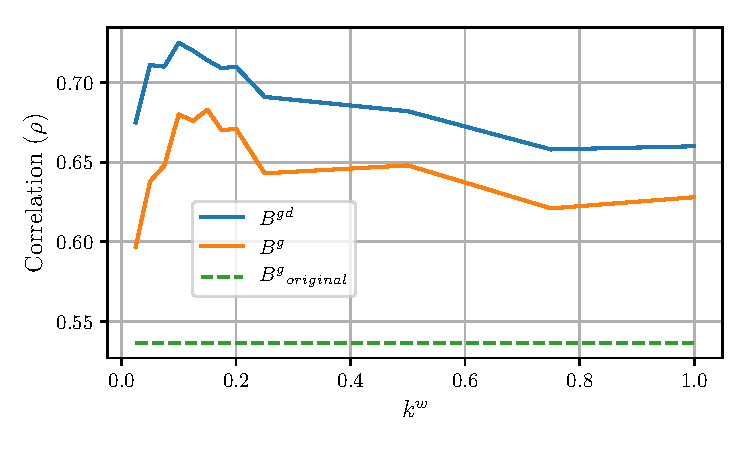
\includegraphics[width=8.0cm]{Figures/gender_correlation.pdf}
	\caption{Average correlations between stereotypical biases and biases calculated from the gender dimension ($B^{gd} = corr(b^s, b^{gd})$, blue line) and from the gender vector ($B^g = corr(b^s, b^{direct})$, orange line) for the imparted word embeddings for $k^w \in [0.025,1.00]$. The reference correlation level that is calculated from the gender vector of the original embedding space ($B^g_{original}$, green dashed line) is also shown.}
	\label{fig:corr}
\end{figure}

 Figure \ref{fig:bias} displays the average direct bias levels of word2vec and imparted embeddings for varying $k^w$. Naturally, imparting gender information in a single dimension does not alter the overall bias in the word embedding, but rather concentrates most of the bias to a single dimension as implied by Figure \ref{fig:corr}. Removing this dimension from the embedding space then considerably reduces the bias, especially for larger $k^w$. Figure \ref{fig:bias} also shows the average direct bias levels of word2vec, imparted and reduced embeddings for varying $k^w$ after debiasing. The bias levels of the full and reduced imparted models (red dashed and dotted lines) are closer in this case, and substantially lower than that for the word2vec model. \textcolor{black}{These results show that learning an embedding space with an explicit gender dimension enhances the performance of the hard-debiasing method.}

\begin{figure}
	\centering
	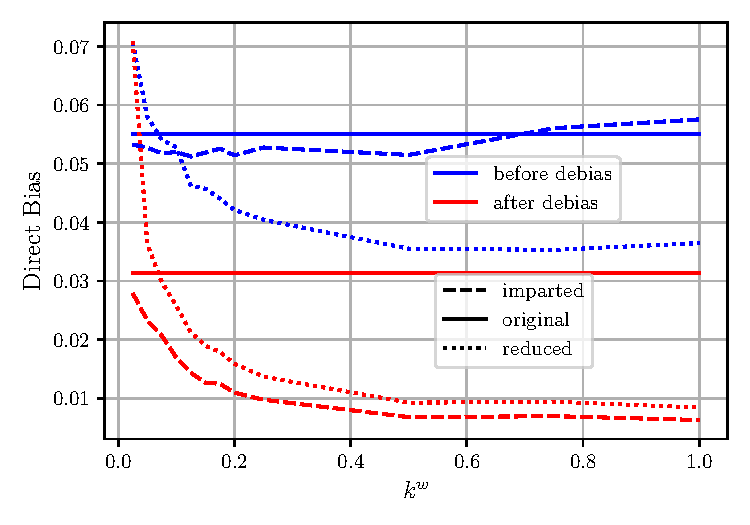
\includegraphics[width=8.0cm]{Figures/gender_bias_reduction.pdf}
	\caption{Average direct bias values of the imparted embeddings (dashed lines) and reduced embeddings (dotted lines) for $k^w \in [0.025,1.00]$ along with the bias values of the original embeddings (solid lines). Results are shown prior to (blue lines) and following (red lines) the hard-debiasing procedure.}
	\label{fig:bias}
\end{figure}

\subsubsection{Bias in Classification}

Hard-debiasing has been suggested to introduce elevated gender bias in high-level classification tasks when compared with original embedding models \citep{prost19biasTextClassif}. Therefore, we coupled gender-imparted embedding models with the \textit{strong-debiasing} method that alleviates this issue by taking $N$ in \eqref{eq:direct_bias} as the entire vocabulary as opposed to gender neutral words \citep{prost19biasTextClassif}. As a gold-standard reference, we use the scrubbing technique \citep{de19biosbias} that removes words characterized as explicit gender indicators from the biographies prior to classification.

Quantitative comparisons of task performance and model fairness, which are measured on BiosBias dataset, were performed on original, scrubbed, hard debiased, strong debiased and imparted - strong debiased embedding models. Table \ref{tab:biosbias} lists classification accuracy, $\text{TPR}_{\text{gap}}$ and $\text{TNR}_{\text{gap}}$ for each model. We find that hard-debiasing reduces classification fairness, as manifested in relatively high $\text{TPR}_{\text{gap}}$ and $\text{TNR}_{\text{gap}}$ values. Strong-debiasing performed on the original word2vec model leads to relatively limited change in classification fairness. Yet, when strong-debiasing is applied to the proposed gender-imparted embeddings (imparted$^{sd}$), it lowers $\text{TPR}_{\text{gap}}$ and $\text{TNR}_{\text{gap}}$ almost to the level of the reference scrubbing method, without a major compromise in accuracy. These results provide further evidence that concentration of gender information to an embedding dimension improves performance of debiasing methods.

\begin{table}
    \centering
	\begin{tabular}{lccc}
	    \hline \hline
        \textbf{Embedding} & \textbf{Acc.} & $\textbf{TPR}_{\textbf{gap}}$ & $\textbf{TNR}_{\textbf{gap}}$ \\\hline \hline %\hhline{===}
        word2vec & 0.717 & 0.094 & 0.0034 \\
        scrubbed & 0.717 & 0.061 & 0.0022 \\
        hard debiased & 0.700 & 0.105 & 0.0037 \\
        strong debiased & 0.699 & 0.087 & 0.0033 \\
        imparted$_{k^w=0.1}^{sd}$ & 0.697 & 0.066 & 0.0022 \\
        imparted$_{k^w=0.5}^{sd}$ & 0.699 & 0.067 & 0.0024 \\
        \hline \hline
	\end{tabular}
	\caption{ Results for the Occupation Classification Task. }
	\label{tab:biosbias}
\end{table}


\section{Conclusion} \label{sec:concl}

In this study, we introduced a new method to enhance interpretability of word embeddings by bidirectional imparting of concepts extracted from lexical sources. The proposed method was implemented for the scalable word2vec algorithm, and semantic concepts were extracted from Roget's Thesaurus and WordNet. A unique component of the proposed method is that, it utilizes both directions along each dimension of the vector space separately, enabling encoding of two different concepts, which can be chosen arbitrarily or chosen as opposite concepts as a special case. 
This allows bidirectional imparting to make more efficient use of the embedding space while increasing encoding flexibility. 
The relative weighting of the interpretability objective against the original word2vec objective was controlled by a tunable parameter $k^w$. Evaluations on word analogy and similarity tests suggest that limiting $k^w$ to a relatively small range ($<0.2$) allows imparted models to attain on par performance with the original embeddings. Thus, a favorable trade-off can be maintained between the goals of enhancing interpretability and maintaining task performance. 

The proposed method was compared against several state-of-the-art methods for improving interpretability of word embeddings. The specific variant considered, WordNet-Bi achieved significantly greater interpretability compared to competing state-of-the-art, particularly in the negative direction. At the same time, evaluations on word similarity/analogy tests as well as sentiment, news, question classification tasks showed that WordNet-Bi does not sacrifice expressive performance of the original embedding model to achieve higher interpretability. Overall, these findings indicate that imparting significantly improves interpretability of word2vec embeddings, without compromising their performance.
%on high-level natural language processing tasks. 

% An important advantage of the imparting method is its ability to concentrate information regarding a desired concept to a pre-defined embedding dimension. Specifically, 
Bidirectional imparting allows to represent opposite concepts in a single dimension as a continuum. As an important demonstration, we used bidirectional imparting to concentrate gender information in a single gender dimension. The gender dimension accurately reflects the stereotypical gender bias as dictated by human judgments. Furthermore, the construction of a gender dimension is shown to be useful to reduce gender bias when coupled with the hard and strong debiasing methods. Collectively, these methods achieved lower levels of gender bias and improved classification fairness. These results highlight the potential of the imparting method in reducing many different types of biases and stereotypes present in word embeddings.

% Here, the imparting method was demonstrated to improve interpretability and reduce gender bias in word2vec embedding models, using concepts from two common lexical sources. That said, imparting through modification of the learning objective is easily adaptable to different embedding algorithms, and to different lexical resources. The imparting framework can also be adopted for goals beyond interpretability enhancement, such as improvement of task performance. If imparting is used to encode task-relevant concepts, similar task performance can be achieved using simpler models with fewer dimensions. In turn, this can offer benefits in terms of memory requirements and computational load. 

\bibliography{NLP_MasterArchive}
\bibliographystyle{acl_natbib}


\clearpage

\appendix

\section{Appendices}



\subsection{Lexical Resources} 
\label{app:lexical_resources}

\begin{table*}
    \centering
	\begin{tabular}{lcccc}
	    \hline \hline
         \multirow{2}{*}{\textbf{Word Counts}} & \multicolumn{2}{c}{\textbf{Roget's Thesarus}}  & \multicolumn{2}{c}{\textbf{WordNet}} \\
         & \textbf{(300 grp.)} & \textbf{(600 grp.)} & \textbf{(300 grp.)} & \textbf{(600 grp.)} \\ \hline \hline %\hhline{====}
         Total & 20978 & 40350 & 26964 & 18965 \\ 
         Unique & 12289 & 19870 & 18123 & 13853 \\
         Average & 69.9$\pm$53.7 & 67.3$\pm$54.6 & 89.9$\pm$74.2 & 31.6$\pm$15.9 \\ \hline \hline %\hhline{====} 
	\end{tabular}
	\caption{Summary statistics of the word-group datasets}
	\label{tab:roget_vs_wordnet}
\end{table*}

In \citet{senel20impart}, Roget's Thesaurus \citep{Roget2008thesaurus} was designated as an external resource.
Here, in addition to Roget's Thesaurus, we also investigate  WordNet \citep{miller95wordnet} to extract semantic word-groups.
In order to extract a specific number of word-groups from WordNet, we partitioned the hierarchical structure starting from the root node, similar to the approach followed in \citet{senel20impart} for Roget's Thesaurus. We followed an iterative approach, where the largest node was divided to its hyponyms in each iteration. Node size was taken as the number of unique words descending from a node after filtering based on the vocabulary extracted from Wikipedia. We discarded the nodes with size less than $\lambda_{min}^w$. Iterations were stopped when the number of nodes exceeded the desired word-group count. Note that the desired word-group count may not be achieved if $\lambda_{min}^w$ is selected too large.
The groups with the smallest number of member words are discarded to achieve desired word-group.

We take $\lambda_{min}^w = 25$ and $\lambda_{min}^w = 15$ for 300 and 600 WordNet word groups, respectively.
Table \ref{tab:roget_vs_wordnet} summarizes the statistics for the constructed word-groups. 

% Please note that our method uses external resources only to select category labels which will be designated as the separate dimensions of the word embedding space. There is no explicit use of knowledge regarding similarity of words that belong each selected category.








\subsection{Training Parameters}
\label{app:training_parameters}

 For the training all imparted models and the original word2vec model, we used \verb|VOCAB_MIN_COUNT| $=100$, \verb|MAX_ITER| $=15$, \verb|WINDOW_SIZE| $=8$, \verb|NEGATIVE| $=15$, \verb|SAMPLE| $=10^{-4}$.
 
 
 
 
 
 
 
 \subsection{Comparison of Imparted Embeddings}
\label{app:impart_comparison}


\begin{figure*}
	\centering
	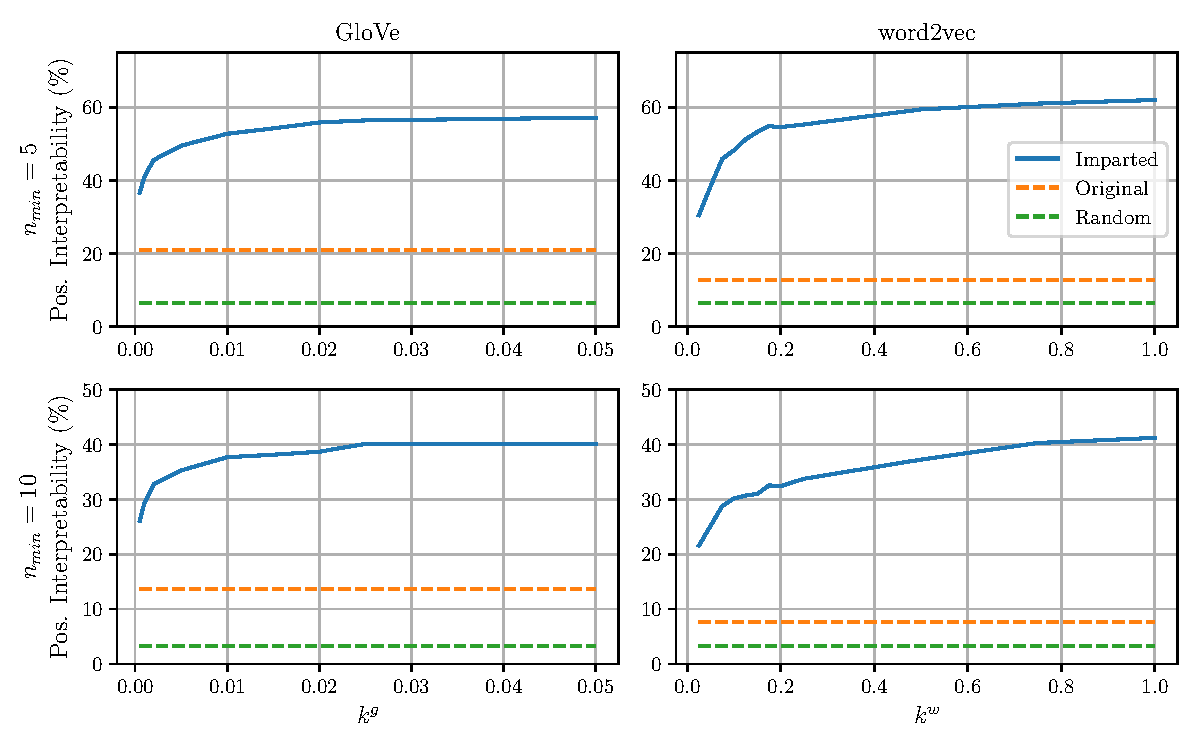
\includegraphics[width=16cm]{Figures/interpretability_glove_vs_word2vec.pdf}
	\caption{Interpretability scores in the positive direction $(IS^+)$ using $n_{min}=5$ (top row) and $n_{min}=10$ (bottom row) for unidirectionally imparted GloVe (left column) and word2vec (right column) algorithms for $k^g \in [0.0005,0.05]$ and $k^w \in [0.025,1.00]$, respectively. Interpretability scores for original embeddings and a random baseline are displayed for comparison as orange and green dashed lines, respectively.}
	\label{fig:g_vs_w2v}
\end{figure*}

Figure \ref{fig:g_vs_w2v} presents the interpretability levels of the unidirectionally imparted GloVe ($k^g \in [0.0005,0.05]$) and word2vec ($k^w \in [0.025,1.00]$) embeddings for $n_{min} = 5$ and $n_{min} = 10$, along with original embeddings and a random baseline. We can see that for both algorithms, imparting substantially improves interpretability. While interpretability of the imparted GloVe embedding does not increase for $k^g$ values beyond 0.03, that for the imparted word2vec embedding is gradually enhanced up to $k^w=1$. Note that the original word2vec embedding has relatively limited interpretability compared to the GloVe embedding.
Yet, for larger $k^w$, interpretability level of the imparted word2vec embedding improves, even surpassing GloVe. 
%These results indicate the viability of the imparting method for the online word2vec algorithm in order to improve interpretability in a memory-efficient and scalable setting.

% \begin{SCfigure*}
\begin{figure*}
	\centering
	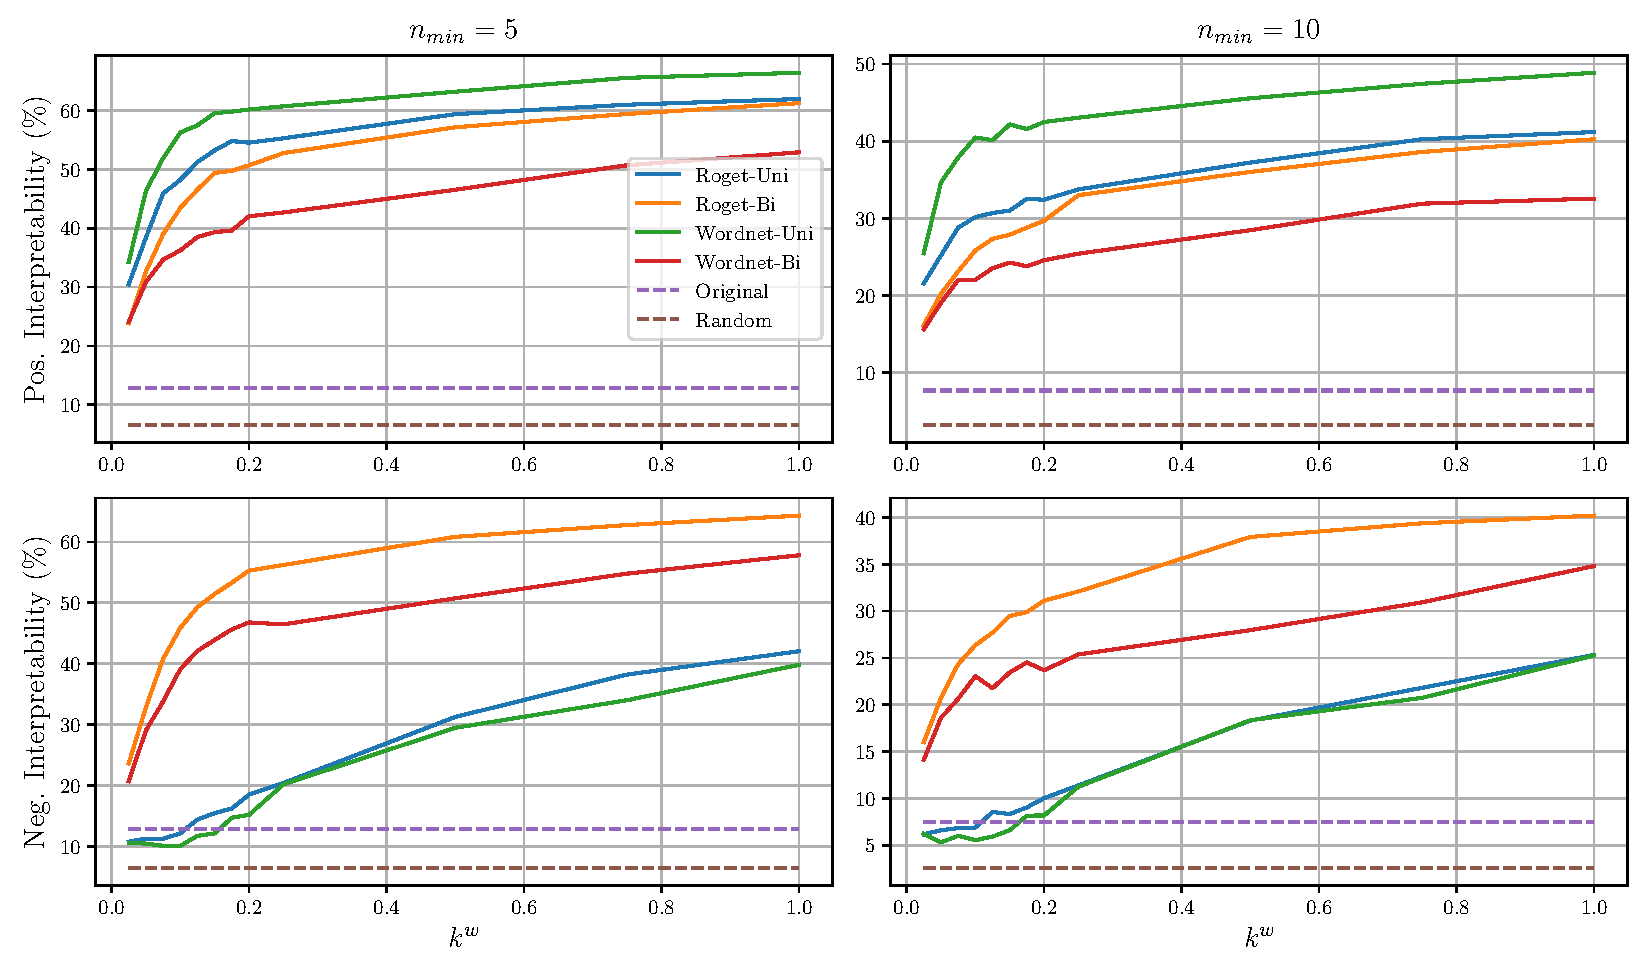
\includegraphics[width=16cm]{Figures/interpretability_wordnet_vs_roget.pdf}
	\caption{Positive (top) and negative (bottom) direction interpretability scores for unidirectionally imparted word2vec embeddings using Roget's Thesaurus (Roget-Uni) and WordNet (WordNet-Uni) and their bidirectionally imparted versions (Roget-Bi, WordNet-Bi) for $k^w \in [0.025,1.00]$ along with the original word2vec embedding and a random baseline for $n_{min} = 5$ (left) and $n_{min} = 10$ (right).}
	\label{fig:wordnet_vs_roget}
\end{figure*}
% \end{SCfigure*}

% \begin{SCfigure*}
\begin{figure*}
	\centering
	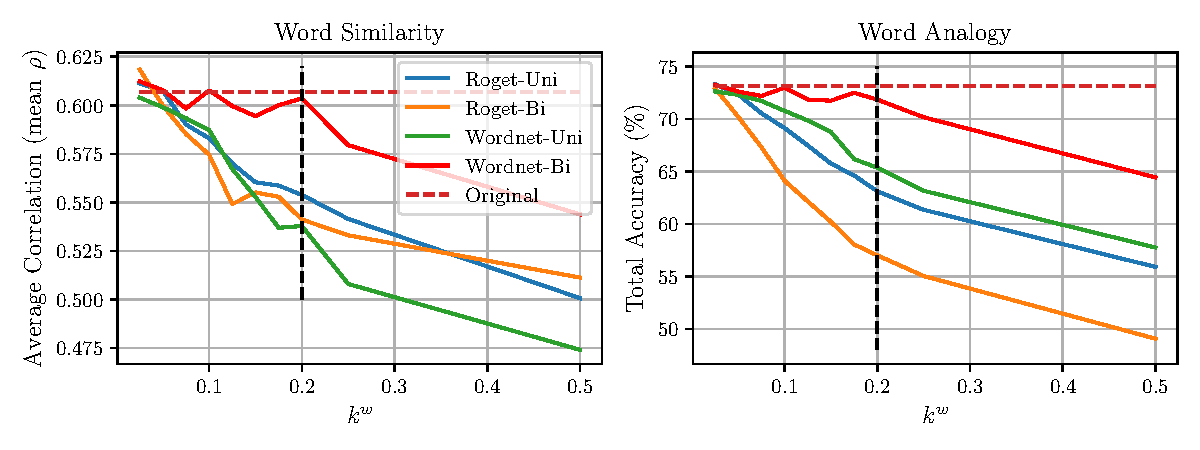
\includegraphics[width=16cm]{Figures/similarity_and_analogy.pdf}
	\caption{Performance of unidirectionally imparted word2vec embeddings using Roget's Thesaurus (Roget-Uni) and WordNet (WordNet-Uni) and their bidirectionally imparted versions (Roget-Bi, WordNet-Bi) for $k^w \in [0.025, 0.500]$ along with the original word2vec embedding on word similarity (left) and word analogy (right) tests. Word similarity results are presented as the average correlations from 13 different word similarity test sets.}
	\label{fig:sim_and_analogy}
\end{figure*}
% \end{SCfigure*}

Figure \ref{fig:wordnet_vs_roget} shows interpretability values of the imparted embeddings for $n_{min} = 5$ and $n_{min} = 10$ \textcolor{black}{in both of the positive and negative directions. It can be seen that bidirectional imparting achieves significantly improved interpretability compared to unidirectional imparting in the negative direction with minimal compromise in the positive direction.}

% Imparting improves interpretability in a controllable manner by offering a tuning parameter $k^w$, that adjusts how heavily the optimization objective weights interpretability against the original goal of capturing semantic relations among words. Naturally, emphasis on interpretability for relatively large values of $k^w$ might lead to suboptimal representation of word semantics. In order to investigate this, we evaluated the imparted embeddings on the intrinsic word analogy \citep{mikolov13word2vec_b} and word similarity \citep{faruqui14communityEval} tests. For analogy tests we use Google analogy dataset\footnote{http://download.tensorflow.org/data/questions-words.txt}. For brevity, word similarity results were averaged across 13 datasets\footnote{Word similarity datasets are: WS-353-ALL, SIMLEX-999, VERB-143, SimVerb-3500, WS-353-REL, RW-STANFORD, YP-130, MEN-TR-3k, RG-65, MTurk-771, WS-353-SIM, MC-30, MTurk-287} on which the evaluations were performed.

Figure \ref{fig:sim_and_analogy} presents the performances of the embeddings on word similarity and word analogy tests. It can be observed that performance on word similarity and analogy tests decreases with increasing $k^w$.  However, for bidirectional imparting of WordNet word-groups, performance is on par with original embeddings for $k^w \leq 0.2$. Taken together, results in Figs. \ref{fig:wordnet_vs_roget} and \ref{fig:sim_and_analogy} suggest that bidirectional imparting of WordNet word-groups at relatively low $k_w$ is the optimal setting for word2vec. While WordNet word-groups somewhat reduce interpretability compared to Roget word-groups in bidirectional setting, they are much better at preserving the semantic structure of the embedding space as suggested by similarity and analogy tests.
 
 
 
 
 
 
 
 
 \subsection{Competing Methods}
 \label{app:competing_methods}
 
 OIWE-IPG was trained on the same corpus as the word2vec embeddings using the default parameters reported in \citep{luo15online} \textcolor{black}{, yielding 300 dimensional vectors}. SOV and Parsimax that work on pre-trained embeddings were performed on the original word2vec embeddings, again using suggested parameters in \citep{faruqui15sparse} and \citep{park17rotated}, \textcolor{black}{resulting in 1000 and 300 dimensional vectors, respectively.} For Word2Sense, we used the publicly available \textcolor{black}{2250 dimensional} pre-trained vectors\footnote{https://github.com/abhishekpanigrahi1996/Word2Sense} due to computational restrictions. \textcolor{black}{For POLAR, we trained two different versions. First, we obtained 1465 dimensional POLAR-large embeddings that were reported in \citep{mathew20polar}, by applying polar transformation on Google's pre-trained word2vec embeddings\footnote{https://drive.google.com/file/d/0B7XkCwpI5KDYNlNUTTlSS21pQmM} using all 1465 antonym pairs. Note that these embeddings were originally trained on a much larger corpus (Google News) with a substantially larger vocabulary (3 million) than our word2vec embeddings. Therefore, POLAR-large embeddings are significantly more expensive than our imparted embeddings in terms of computational and linguistic resources. Second, we obtained 500 dimensional POLAR-small embeddings that are more comparable to imparted embeddings in terms of model dimensionality and resource usage, by performing the polar transformation on our original word2vec embeddings using the default parameters\footnote{https://github.com/Sandipan99/POLAR}.} 
 
 
 
 
 
 
 

\subsection{Classification Tasks}
\label{app:clf_tasks}

The classification tasks are described in detail below:
\begin{itemize}
    \item \textbf{Sentiment Analysis:} A sentence-level binary classification task using the Stanford Sentiment Treebank consisting of thousands of movie reviews \citep{socher13treebank} and their sentiment scores. The development and training sets in the original dataset were aggregated, and reviews with neutral scores were removed (i.e., scores between 0.4 and 0.6). The resulting dataset contained 7407 training and 1751 test samples.
    
    \item \textbf{Question Classification (TREC):} A question-level multinomial classification task using the TREC dataset \citep{li06learning} consisting of six different types of questions (person, location, entity, number, description, abbreviation). This dataset consisted of 5452 training and 500 test questions.
    
    \item \textbf{News Classification:} Following \citep{faruqui15sparse}, three news-level binary classification tasks were considered using the 20 Newsgroup dataset\footnote{http://qwone.com/~jason/20Newsgroups}. The following news topics were considered (training/test sample counts): 1) Religion: atheism vs christian (1079/716); 2) Sports: baseball vs hockey (1192/796); 3) Computers: IBM vs Mac (1162/775).
\end{itemize}

For these high-level NLP tasks, we took the average of the word vectors in input text (can be a sentence, question or news) as input features and trained an SVM classifier that was tuned using 5 fold cross-validation on the training sets. 






\subsection{Performance of Gender Biased Embeddings}

A potential risk of debiasing on gender-imparted models is undesirable loss of semantic structure in the embedding space that might compromise task performance. To rule out this risk, we evaluated the embeddings in the gender-bias experiments on intrinsic tests and downstream classification tasks. For the imparted and reduced embeddings, we averaged the results across $k^w$. Table \ref{tab:gender_performance_tests} shows that all the evaluated embeddings perform nearly as good as the original embeddings on all tasks, except a slightly reduced performance on computer news classification task. These results indicate that debiasing of gender-imparted embeddings successfully preserves semantic structure of the embedding space.

\begin{table*}
    \centering
	\begin{tabular}{lcccccc}
		\hline \hline 
		\multirow{2}{*}{\textbf{Task}} & \multicolumn{3}{c}{\textbf{before debias}} & 
		\multicolumn{3}{c}{\textbf{after debias}} \\
		 & \textbf{word2vec} & \textbf{imparted} & \textbf{reduced} & \textbf{word2vec} & \textbf{imparted} & \textbf{reduced} \\ \hline \hline %\hhline{======}
	    Sem. Anlg. & 79.87 & 79.00 $\pm$ 0.50 & 79.16 $\pm$ 0.50 & 78.65 & 78.92 $\pm$ 0.57 & 78.99 $\pm$ 0.61 \\
	    Syn. Anlg. & 67.63 & 66.39 $\pm$ 0.99 & 66.48 $\pm$ 1.01 & 67.46 & 66.42 $\pm$ 0.96 & 66.43 $\pm$ 1.00 \\ 
	    \hline %\hhline{------}
	    Word Sim. & 60.68 & 60.08 $\pm$ 0.66 & 60.21 $\pm$ 0.52 & 60.64 & 60.12 $\pm$ 0.67 & 60.28 $\pm$ 0.53 \\
	    \hline %\hhline{------}
	    Sent. Anly. & 80.30 & 79.95 $\pm$ 0.36 & 79.94 $\pm$ 0.33 & 79.84 & 79.99 $\pm$ 0.37 & 79.98 $\pm$ 0.41 \\ \hline %\hhline{------}
	    Quest. Clf. & 85.80 & 84.63 $\pm$ 0.59 & 86.00 $\pm$ 0.92 & 86.20 & 86.27 $\pm$ 0.74 & 86.03 $\pm$ 0.80 \\ \hline %\hhline{------}
	    Sports News & 95.85 & 95.33 $\pm$ 0.27 & 95.34 $\pm$ 0.25 & 95.10 & 95.33 $\pm$ 0.27 & 95.33 $\pm$ 0.29 \\
	    Relig. News & 87.01 & 86.19 $\pm$ 0.61 & 86.10 $\pm$ 0.57 & 86.03 & 86.24 $\pm$ 0.59 & 86.18 $\pm$ 0.59 \\
	    Comp. News & 81.55 & 78.74 $\pm$ 0.84 & 78.73 $\pm$ 0.99 & 78.84 & 78.68 $\pm$ 0.83 & 78.63 $\pm$ 0.81 \\ \hline \hline %\hhline{======}
	\end{tabular}
	\caption{Results of embeddings from gender bias experiments on the performance evaluation tests. }
	\label{tab:gender_performance_tests}
\end{table*}








\subsection{Hybrid Gender and Interpretability Imparted Embeddings}

\begin{table}
    \centering
	\begin{tabular}{lccc}
		\hline \hline 
		\textbf{Task} & \textbf{$\setlength{\thickmuskip}{0mu}k^w=0.1$} & \textbf{$\setlength{\thickmuskip}{0mu}k^w=0.2$} & \textbf{$\setlength{\thickmuskip}{0mu}k^w=1$}\\ \hline \hline %\hhline{======}
	    Semantic Anlg. & 79.07 & 78.13 & 73.25 \\
	    Syntactic Anlg. & 66.61 & 65.17 & 45.58 \\ 
	    \hline %\hhline{------}
	    Word Sim. & 60.62 & 59.11 & 48.94 \\
	    \hline %\hhline{------}
	    Sentiment Anly. & 80.41 & 79.55 & 79.84 \\ \hline %\hhline{------}
	    Question Clf. & 84.60 & 85.00 & 84.20 \\ \hline %\hhline{------}
	    Sports News & 96.11 & 95.73 & 95.73 \\
	    Religion News & 85.89 & 87.43 & 88.55 \\
	    Comput. News & 81.42 & 81.03 & 79.74 \\\hline
	    Interp.$^+_{n_{min}=5}$ & 36.88 & 41.22 & 54.28 \\
	    Interp.$^-_{n_{min}=5}$ & 38.47 & 44.79 & 58.50 \\
	    Interp$^+_{n_{min}=10}$ & 22.41 & 24.17 & 34.07 \\
	    Interp.$^-_{n_{min}=10}$ & 22.49 & 23.89 & 35.43 \\\hline
	    Gender B.$_{reduced}$ & 0.0470 & 0.0403 & 0.0441 \\
	    Gender B.$_{debiased}$ & 0.0168 & 0.0122 & 0.0148 \\ 

	    \hline \hline %\hhline{======}
	\end{tabular}
	\caption{ Results of Evaluation Tests for the Hybrid Gender and Interpretability Imparted Embeddings.}
	\label{tab:gender_plus_wordnet}	
\end{table}

Finally, we demonstrated the feasibility of the proposed approach for concurrent gender and interpretability imparting. To do this, we obtained a hybrid model where the first dimension was encoded with gender word-groups and the remaining 299 dimensions were bidirectionally imparted with word-groups extracted from WordNet. Evaluation on gender bias, interpretability and task performance were repeated on this hybrid model. We find that the hybrid embeddings perform similarly to WordNet-Bi in terms of interpretability and task performance, for all evaluations and for all $k^w$ (Table \ref{tab:gender_plus_wordnet}). We also find that the hybrid embeddings perform similarly to gender-imparted embeddings in gender bias evaluations (Table \ref{tab:gender_plus_wordnet}). These results indicate that the proposed bidirectional imparting method enables gender debiasing and interpretability enhancement simultaneously in embedding models without compromising task performance.

\end{document}
